\setcounter{chapter}{4}
\chapter{Überlandflug Aufgaben - Navigieren mit\textsf{XCSoar}}\label{cha:tasks}\index{Aufgabe}\index{Tasks}

\textsf{XCSoar} bietet ein ausgefeiltes, komplettes Aufgabenmanagementsystem, mit dem Aufgaben vor und während des Fluges erstellt, editiert und auch gelöscht werden können.

Die Wendepunkte können vollautomatisch angeflogen und umgestellt werden, wobei die Kartendarstellung automatisch hinein- bzw. herausgezoomt werden kann. Ein rein manuelles  Anwählen und Umschalten ist aber ebenso möglich.

Dieses Kapitel beschreibt weiterhin die Benutzung von \textsf{IGC} Loggern mit\textsf{XCSoar}

Intern werden drei Aufgabentypen (modi)  unterschieden
\begin{description}
\item[Deklarierte Aufgabe] Dies ist der eigentliche Überlandflug-Modus, bei dem ein Startpunkt, ein
    Zielpunkt und mehrere Wendepunkte deklariert sein können. Die Wendepunkte müssen in der
    angegeben Reihenfolge angeflogen werden. (Leistungsflug)\index{task!Leistungsflug}
\item[Gehe zu - Aufgabe] Ein Flug auf exakt ein einziges Ziel zu. (Irgendein Flug)\index{task!Zielflug}
\item[Abort - Aufgabe] Hier wird "frei" durch die Gegend geflogen, ohne einen Wegpunkt als  Ziel
    deklariert zu haben. (Lustflug)\index{task!Lustflug}
\end{description}

 Beachte, daß im Gehe zu- und im Abort - Modus  die  evtl.\ abgebrochene Aufgabe \textsl{jederzeit} wieder \tip aufgenommen werden kann, dies unter Beibehaltung sämtlicher bisher aufgenommenen Berechnungen und Statistiken.

\section{Gehe zu Aufgabe}\index{Aufgabe!Gehe zu-Typ}\index{Task!Gehe zu}

Gehe zu-Aufgaben können erstellt werden, indem man einen Wegpunkt auf der Karte markiert und anschließend auf der Wegpunkt-Detailfenster mit "Gehezu" bestätigt.  Alternativ kann auch über den "Alternative" Dialog zu einem Wegpunkt gelangt werden, welcher anschließen d mit Gehe zu festgelegt wird.

Während des Gehe zu-Modus kann eine vorher abgebrochene Aufgabe wie folgt fortgesetzt werden:
\begin{quote}
\smenus{Nav}\blink\smenut{Aufgabe}{Fortsetzen}
\end{quote}
\index{Aufgabe!Fortsetzen}
\subsection{Automatik-Gehe zu}\index{Automatik-Gehe zu}\index{Heimatflugplatz!Automatik}

Wenn keine deklarierte Aufgabe geladen ist, dann wird nach dem Start unverzüglich in den Gehe zu Mode geschaltet. Hierbei wird der Startplatz oder aber (falls es z.B. eine Wiese war, von der man mit einer  Wilga im F-Schlepp gestartet ist), der nächstgelegene landbare Flugplatz automatisch als Ziel in den Rechner eingefügt.

Egal, ob eine Aufgabe deklariert wurde, oder nicht, es wird grundsätzlich ein Startpunkt erfaßt, welcher für spätere Benutzung während des Fluges in der Wegpunktliste erscheint und ganz normal  verwendet werden kann.  \todonum{wird der auch gespeichert? wo ?}

\section{Aufgaben erstellen und Bearbeiten}\index{Aufgabe!Erstellen}\index{Aufgabe!Bearbeiten}

Aufgaben können auf unterschiedliche Weise erstellt und editiert  werden. Manche Methoden eigentlich mehr für die Bearbeitung und Erstellung vor dem Flug,  andere erlauben es eine Aufgabe während des Fluges zu ergänzen bzw. zu verändern.

Aufgaben können in Dateien (Files) gespeichert werden um später geladen zu werden oder aber um zwischen verschiedenen Geräten hin und her kopiert zu werden. Alle\textsf{XCSoar} Plattformen sind Dateiformatskompatibel d.h.\  jede Aufgabe kann auf jedem\textsf{XCSoar} erstellt, geflogen und gespeichert werden. (\textsf{Pocket PC, Altair, PC, Android(?), MAC(?)}).\todonum{Geht das bei MAC und Android auch?}

\tip Es ist möglich (und sinnvoll) eine Standard-Aufgabe zu erstellen und zu speichern und diese  Aufgabe beim jedem Start von\textsf{XCSoar} automatisch laden zu lassen.

Eine Anwendung dieser Standardaufgabe ist zum Beispiel, einen Wegpunkt  als Heimatflughafen zu deklarieren. D.h.,  der Heimatflugplatz ist anschließend grundsätzlich automatisch als Ziel eingestellt, wenn man einfach nur durch die Gegend fliegt.

Die Möglichkeiten, Aufgaben zu erstellen sind wie folgt:
\begin{itemize}
\item Benutzen des Aufgabeneditor-Dialogs
\item Auswählen eines Wegpunkt es von der Karte und hinzufügen zur Aufgabe über den Wegpunkt Detail-Dialog.
\item Laden einer Aufgabe aus einer Datei.
\end{itemize}

\tip Aufgaben in einer Datei zu sichern und anschließend wieder zu laden ist sehr sinnvoll,  will man zum Beispiel mit mehreren Piloten eine gleiche Aufgabe fliegen oder aber im Wettbewerb ist, wo im  allgemein die Aufgaben vorher deklariert und eingegeben werden.

Entscheidend hierbei ist, daß lediglich eine Person die Aufgabe eingeben muss und hinterher per Copy \& Test Bluetooth oder Kabel kopieren kann.

\textsf{XCSoar} sichert die aktuelle Aufgabe beim Herunterfahren und lädt die gleiche Aufgabe wieder beim Neustart.  Die Wegpunkte einer Aufgabe sind sogar gesichert, wenn die Wegpunktdatei gewechselt wird. d.h., wenn eine Aufgabe gespeichert wird, anschließend das Wegpunktfile gewechselt wird, die gleiche Aufgabe wieder geladen  wird, wenn die Wegpunkte, welche in der Wegpunktdatei  fehlen automatisch durch die Wegpunkte aus der Aufgabe ergänzt.

\section{Wegpunkt-Info Dialog}\index{Wegpunkt!Details}

Der Wegpunkt-Info-Dialog beschreibt die Details der Wegpunkte  und bietet Navigations-Optionen wie zum Beispiel \textsf{Gehe zu}, \textsf{Einfügen} oder \textsf{Anhängen} an einer Aufgabe.

Weiterhin kann über diesen Dialog ein Wegpunkt als Heimatflughafen eingegeben werden.

Dies kann über mehrere Wege erfolgen:
\begin{itemize}\itemsep=1em
\item Über den Aufgabeneditor: \index{Wegpunkt!Anwahl}
\begin{quote}
\bmenu{Nav}\blink\bmenu{Aufgabe}\blink\bmenu{Wendepunkt}\blink\bmenu{Wendepunkt  hinzufügen} und \bmenu{Wendepunkt auswählen} wählen.
\end{quote}
\item
Vom Menü \bmenu{Info}\blink\bmenu{Info}\blink\bmenu{Waypoint Details}  und anschließend auf \bmenu{Gehezu}
\item
Über das Menü
\begin{quote}
\bmenu{Info}\blink\bmenu{Info}\blink\bmenu{Info}\blink\bmenu{Naher Wendepunkt}
\end{quote}
und auf der sich öffnenden Detailseite des zugehörigen Wepgpunktes unten \bmenu{Gehezu} anwählen.

Falls im Verschiebe Modus befindlich, kann das Menü \bmenu{Naher Wendepunkt} auch durch Verschieben der Moving Map an das Fadenkreuz  an den Wendepunkt ausgewählt werden.
\item%[\Large{$\bullet$}]
Vom Wegpunkt-Auswahlmenü \bmenu{Nav}\blink\bmenu{Wegpunkt Liste} und \bmenu{Auswählen}
(Hier kann mittels eines einiger Filters besonders schnell und elegant jeder beliebige Wegpunkt auf schnellstmögliche Weise ausgewählt werden. Sehr effektiv, wenn man nicht nur den nächst möglichen Wegpunkt anwählen will.)
\item
Ist der gewünschte Wegpunkt auf dem Moving Map Bildschirm im entsprechenden Kartenmaßstab  sichtbar, einfach \textsl{einmal} anklicken und auf der sich öffnenden Detailseite des zugehörigen Wepgpunktes unten \bmenu{Gehezu} anwählen.
\end{itemize}

Der Wegpunktdetail-Dialog enthält zwei maßgebliche Seiten, welche über \button{$>$} und  \button{$<$} weiterschaltbar sind. Je nach dem, ob noch weitere Informationen zum Wegpunkt vorliegen, erscheinen Seiten mit weitere Details hierzu.

\subsection*{Wegpunkt Details}\index{Wegpunkt!Details}

Auf dieser Seite werden Details zum Wegpunkt wie z.B.\ Funkfrequenz, Länge der Bahn, Höhe, Art der Bahn, Namen, Peilung (Bearing), Sonnenuntergang Entfernung zum Wegpunkt. etc.\ angegeben.

Zusätzlich befindet sich ein Button \button{Gehezu} um direkt zu diesem Punkt zu navigieren.  Dieser Button bricht die aktuelle Aufgabe, sofern vorhanden, ab.
\begin{center}
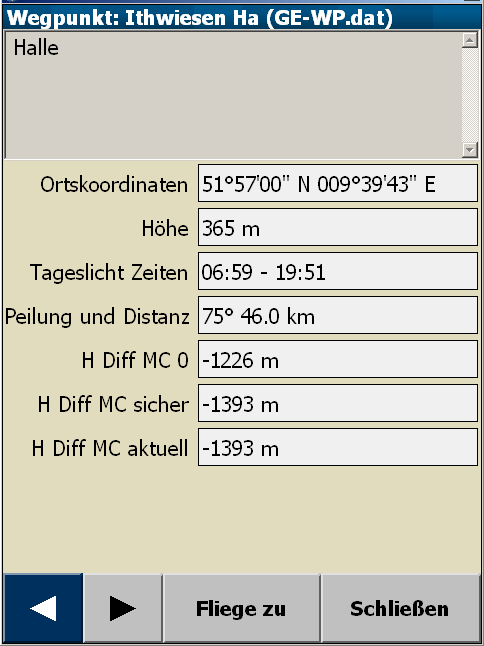
\includegraphics[angle=0,width=0.8\linewidth,keepaspectratio='true']{figures/dialog-waypointdetails0.png}
\end{center}

Wie bereits oben erwähnt, zeigt der Wegpunkt-Info-Dialog drei Höhendifferenz-Angaben zum Erreichen des Wegpunktes, welche hier unten beschrieben werden:

\begin{description}
\item[Höhenunterschied MC 0] Benötigte Höhendifferenz bei MacCready Einstellung null
\item[Höhenunterschied MC Sicherheit] Benötigte Höhendifferenz bei MacCready Einstellung Sicherheits MC (Hierzu auch Abschnitt \ref{sec:Safetyfactors})
\item[Höhenunterschied MC aktuell] Benötigte Höhendifferenz beim  aktuell eingestellten MacCready Wert
\end{description}

Über die Buttons \button{$<$} und \button{$>$} in der linken unteren Ecke des Fensters können weitere Seiten mit Informationen über den aktuellen Wegpunkt angewählt werden.


\subsection*{Flugplatz Informationen}
Diese Seite kann -sofern Daten zum Flugplatz vorhanden- etliche Hinweise und Details zu Flugplätzen enthalten. Insbesondere sind hier enthalten Details zur Landebahn, Landebahnrichtung, Höhe, Frequenz usw.

\begin{center}
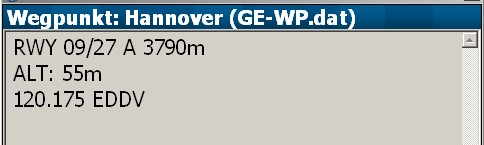
\includegraphics[angle=0,width=0.8\linewidth,keepaspectratio='true']{figures/dialog-waypointdetails1.png}
\end{center}

\subsection*{Satelliten Photo}
\halt Sofern vorhanden, kann hier ein Satellitenfoto des Flugplatzes eingefügt und angezeigt werden.
\todonum{Has this feature been removed, or is it because I haven't loaded the satellite images into the waypoint datafile?
Where is this documented?}

\begin{center}
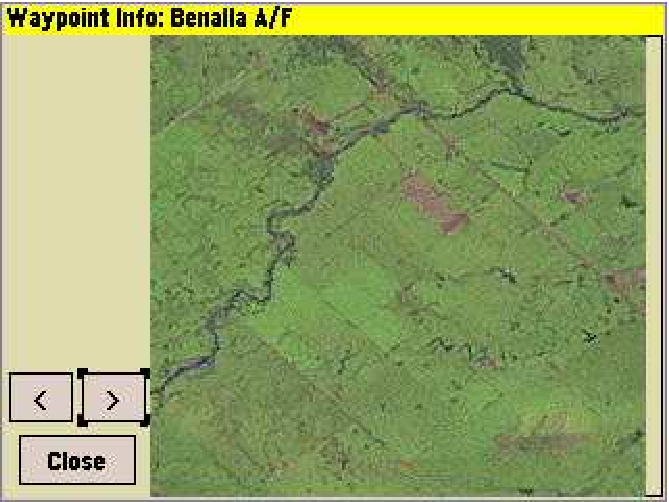
\includegraphics[angle=0,width=0.8\linewidth,keepaspectratio='true']{figures/dialog-waypointdetails2.pdf}
\end{center}


\section{Wegpunkt-Auswahl-Dialog}\label{sec:waypoint-selector-dialog}

Der Wegpunkt-Auswahl-Dialog ist \textsl{der} Dialog, von dem aus Wendepunkte die in einer Datenbank (Datei) enthalten sind, ausgewählt werden kann.

Das kann auf zwei Arten erfolgen:
\begin{itemize}
\item  Vom Menü \smenus{Nav}\blink\smenut{Wegpunkt}{Liste}
\item  oder aber mittels einer Geste: Runter-rechts\gesture{Runter -Rechts}.
\end{itemize}

Die Wegpunktlisten-Auswahlseite bietet einen Satz an von vier Filtern, um die Auswahl der entsprechenden Wegpunkte schneller und effizienter zu machen. Diese Filter können einzeln, gar nicht oder alle zusammen benutzt werden, umso die Auswahl eines Wegpunkt  einzugrenzen.

Folgende Wegpunktfilter sind vorhanden:

\begin{description}
\item[\button{Name}] Dieser Filter bietet eine sehr schnelle Möglichkeit, Wegpunkte anhand des Namens herauszufiltern.
\item[\button{Distanz}] Über diesen Filter werden die Wegpunkte nach der Entfernung angeordnet. Die nächstgelegene Mittelpunkte werden an die Spitze der Liste gesetzt.
\item[\button{Richtung}] Hiermit werden Wegpunkt ausgewählt, welche in der entsprechenden gewünschten Richtung liegen.
    Ein besonderer Filter hierbei ist der Heading-Filter (\textsf{HDG(0$^\circ$)}) welcher nur Wegpunkte anzeigt, die sich in einem Winkel von $\pm 30\circ$ zur Flugrichtung befinden.
\item[\button{Typ}] Über diesen Filter werden die Wegpunkte anhand ihrer Eigenschaft (Flugplatz, Landefeld, Startpunkt, oft benutzt, enthalten im Wegpunktdatei 2), usw. ausgewählt.
\end{description}

Wenn die Filterung nach Namen und gilt gewählt wird, ist die Ergebnisliste nach dem Namen geordnet. Wenn (auch zusätzlich) die Wegpunkte nach Entfernung oder Richtung gefiltert werden, dann erfolgt die Sortierung der Wegpunkte grundsätzlich als erstes nach der Entfernung.
D.h., der als nächste gefundene Wegpunkt wird immer an die Spitze der Liste gesetzt.

\begin{center}
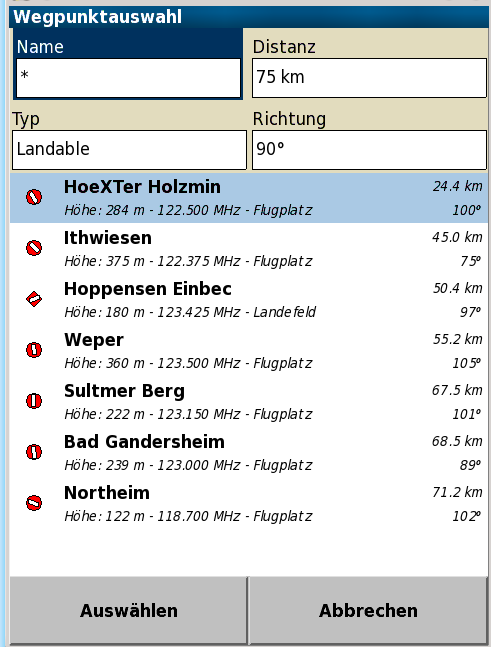
\includegraphics[angle=0,width=0.8\linewidth,keepaspectratio='true']{figures/dialog-waypointselect.png}
\end{center}

Diese Ergebnisliste kann durchgescrollt werden, wenn Sie Einträge mehr als auf einer Seite dargestellt werden können. Um zu scrollen, einfach mit dem Finger auf dem TouchScreen hoch und runter, oder aber die Drehknöpfe beim Altair benutzen, alternativ mit der Maus ans Ende oder Spitze der Liste fahren.

Je nachdem aus welcher Situation die Wegpunktauswahl aufgerufen wurde, kann das Verhalten unterschiedlich sein. Normalerweise bringt die Anwahl eines Wegpunktes aus der Liste  direkt das Wegpunkt-Detail-Fenster.

\section{Aufgabenverwaltung }\label{sec:task-manager-dialog}
Die Aufgabenverwaltung wird benutzt, um Aufgaben zu erstellen, zu löschen, zu speichern und zu deklarieren. Sie ist in der Zwischenzeit massiv bearbeitet und komplett neu gestaltet worden.

Gegenüber früheren Versionen von \textsf{XCSoar} befindet sich so gut wie nichts mehr an der gewohnten und üblichen Stelle; das Arbeiten mit der neuen Version hat sich jedoch erheblich vereinfacht und ist deutlich komfortabler, übersichtlicher und schneller geworden.
 
\menulabel{ \bmenut{Nav}{1/2}\blink \bmenus{Aufgabe} }
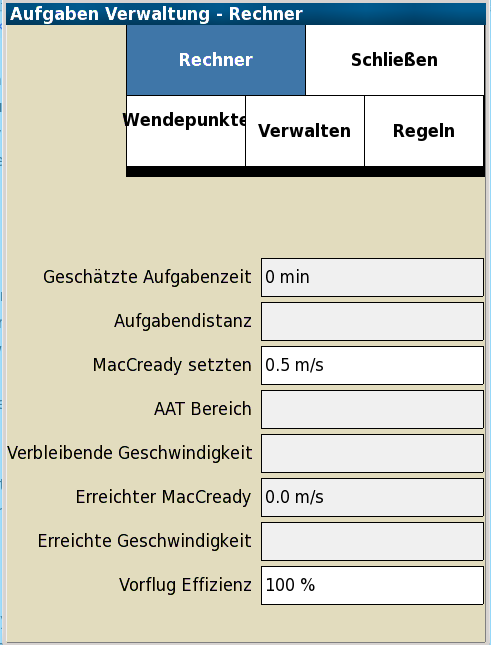
\includegraphics[keepaspectratio,width=0.75\textwidth]{figures/dialog-taskcalculator.png}
Die Startseite der Aufgabenverwaltung ist der Rechner. Hier werden diverse berechnete Werte angezeigt, die aktuelle Aufgabe betreffen und im Detail weiter unten beschrieben werden.

Weiterhin stehen folgende Buttons zur Verfügung:  \button{Rechner}, \button{Wegpunkt}, \button{Verwalten}, und \button{Regeln}, sowie selbstverständlich \button{Schließen}, 
um die Aufgabenverwaltung zu schließen.

\subsection*{Wegpunkt}
Der Button  \button{Wegpunkt} zeigt eine Liste der aktuell in der jeweiligen Aufgabe bestimmten Wegpunkt. Wenn kein Wegpunkt In der aktuellen Aufgabe gelistet ist, gibt es nur eine einzige Option, und zwar die, einen Wegpunkt hinzuzufügen: "Wegpunkt hinzufügen"

Durch Drücken auf die graue "Wegpunkt hinzufügen" Schaltfläche wird die Wegpunkt Auswahl gestartet (siehe oben).  Ein hier ausgewählter Wegpunkt erscheint anschließend in der Aufgabe.

\subsection*{Verwaltung}

Durch Drücken auf den Button \button{Verwaltung} wird die Verwaltung der Aufgaben geöffnet, hierbei erscheinen vier große Schaltflächen:

\begin{itemize}
\item \button{Neue Aufgabe} Löscht die aktuelle Aufgabe und setzt die Regeln auf die Standardwerte.
\item \button{Anmelden} Wenn ein externer Bürger angeschlossen ist, wird hiermit die aktive Aufgabe an den Logger übertragen und somit deklariert.
\item \button{Durchsuchen} Zeigt eine Liste aller gespeicherten Aufgaben, und erlaubt es, Aufgaben zu laden. Beachte, daß diese Option die aktuelle Aufgabe löscht.
\item \button{Speichern} Sichert die aktuelle Aufgabe. Nachdem die Schaltfläche berührt wurde, wird der Not aufgefordert, einen Namen zu vergeben, unter dem die Aufgabe gespeichert wird und wieder geladen werden kann.
\end{itemize}

\subsection*{Regeln}\index{Regeln}

Die Werte, die bei Anklicken des Buttons \button{Regeln} erscheinen, hängen vom Typ der Aufgabe ab, die vorher erstellt wurde.

Durch Anklicken der jeweiligen weiß hinterlegten Werte wird ein Untermenü geöffnet, auf dem diese Werte entsprechend geändert werden können. Die di^^versen Aufgabentypen werden in einem Abschnitt weiter unten besprochen.

Ein erneutes Drücken des Buttons  \button{Regeln} öffnet eine Kartenansicht der aktuellen Aufgabe. Erneutes Anklicken des Buttons führt wieder zu den einzelnen werden.

\subsection*{Aufgabentypen}\index{Aufgabentypen}

\textsf{XCSoar} unterstützt derzeit folgenden verschiedenen Aufgabentypen:
Racing, AAT und FAI Abzeichen/Rekorde.

Eine Kurzbeschreibung der diversen Aufgabentypen erfolgt erfolgt unten. In diesem Handbuch sollen aber nicht die kompletten FAI Regeln wiederholt werden. Für eine ausführliche Beschreibung der jeweiligen Aufgabentypen kann  auf der Homepage der FAI nachgeschaut werden: \url{http://www.fai.org}.

\begin{description}
\item[Racing] Eine  "racing" Aufgabe besteht aus einem Startpunkt, mehreren Wendepunkt,  und einem Zielpunkt, welche in vorgeschriebener Reihenfolge und so werden müssen. (Wenn hier unter "Regeln" FAI Start/Zielregeln auf "Ein" geklickt ist dann sind keiner weiteren Optionen verfügbar FAI-Regeln sind fix).\index{Regeln!Racing}
        \begin{itemize}
            \item max. Abfluggeschwindgkeit:     Hier wird die maximale Abfluggeschwindigkeit, die vom Veranstalter vorgegeben wird, eingestellt. Wenn die Abfluggeschwindigkeit nicht limitiert ist, sollte der Wert "0"  eingestellt werden.
            \item Maximale Abflughöhe: Hier wird die maximale Abflughöhe eingetragen, die der Veranstalter vorgibt.   Wenn die Abflughöhe nicht limitiert ist, sollte hier "0" eingetragen werden.
            \item Abflughöhe bezogen auf: Hier wird eingetragen, ob die Abflughöhe auf den Startpunkt (AGL) oder aber auf  Meereshöhe (MSL) bezogen ist.
            \item Minimale Ankunftshöhe:  Dies ist die vom Veranstalter vorgegebene minimale Ankunftshöhe. Ist keine vorgegeben, so sollte hier "0"  stehen.
            \item Zielhöhenref.:  Hier wird eingetragen, ob die Ankunftshöhe auf den  Startpunkt (AGL) oder aber auf  Meereshöhe (MSL) bezogen ist.
            \item FAI Start/Zielregeln: Wenn hier ein angeklickt wurde,  dann  gelten die FAI-Regeln. D.h., es gibt keine maximale Starthöhe und keine maximale Abfluggeschwindigkeit. Die Zielhöhenreferenz ist bezogen auf den Startpunkt (AGL) und die minimale Ankunftshöhe beträgt 1000m oberhalb der Starthöhe. \todonum{richtig??}
    \end{itemize}
\item[AAT]
 Dieser Aufgabentyp beschreibt eine  Aufgabe, bei der um verschiedene Wendepunkte herum gewisse Flächen (Kreise, Segmente, ö.ä) gezeichnet sind, in denen jeweils mindestens ein Punkt gelegt werden muß werden muss.
 Es wird eine \textsl{mindestens} zu fliegende Zeit vorgegeben.
    \begin{itemize}\index{Regeln!AAT}
            \item AAT min. Zeit:  Diese Zeit muß mindestens geflogen werden, um eine Wertung ohne Punktabzug zu bekommen. Eine Ankunft am Zielpunkt, bevor die Mindestzeit abgelaufen ist, wird in der Regel mit Strafpunkten bewertet und ist in aller Regel mit einem schlechteren Schnitt versehen.
        	\item Max. Abfluggeschwindigkeit: Identisch wie bei der Racing-Aufgabe
        	\item Maximale Abflughöhe: Identisch wie bei der Racing-Aufgabe
        	\item Abflughöhe bezogen auf: Identisch wie bei der Racing-Aufgabe
        	\item minimale Ankunftshöhe: Identisch wie bei der Racing-Aufgabe
        	\item Zielhöhenref. : Identisch wie bei der Racing-Aufgabe
        	\item FAI Start/Zielregeln: Identisch wie bei der Racing-Aufgabe
    \end{itemize}
\item[FAI Abzeichen/Rekorde] Diese Aufgaben Typ erlaubt ausschließlich FAI- Start, Wende- und Zielpunkte gemäß der o.g. Regeln auf der FAI-Homepage.\index{Regeln!Abzeichen, Rekorde}
\end{description}

Nachdem eine entsprechende Aufgabe ausgewählt wurde und Start- und Zielregeln definiert wurden (wie oben beschrieben), ist es notwendig die Eigenschaften jedes Wegpunktes in der Aufgabe zu beschreiben. Wegpunkte können Startpunkte, Wendepunkte oder Zielpunkte sein.

Dies erfolgt, indem man auf die \bmenu{Wegpunkt} Schaltfläche klickt und anschließend den gewünschten Wegpunkt in der Liste auswählt. Entweder durch Doppelklick oder aber durch den Button \button{Bearbeiten} wird ein entsprechendes Fenster geöffnet, auf dem die Eigenschaften (Startpunkt, Zielpunkt, Wendepunkt, AAT-Punkt und -Radius) zur Bearbeitung bereit stehen.

\begin{itemize}
\item \bmenu{Vorheriger} Hiermit wird zum vorherigen Wegpunkt innerhalb der Aufgabe gesprungen.
\item \bmenu{Nächster} Hiermit kann zum nächsten Wegpunkt innerhalb der Aufgabe gesprungen werden.
\item \bmenu{Schließen} Verläßt das Bearbeiten-Menü.
\item \bmenu{Details} Öffnet das Wegpunkt-Detailfenster.
\item \bmenu{Entfernen} Hiermit kann ein Wegpunkt aus einer Aufgabe entfernt werden.
\item \bmenu{Versetzen} Ermöglicht es, den Wegpunkt Innerhalb dieser Aufgabe zu versetzen. Ein Anklicken öffnet die Wegpunkt Auswahl.
\item \bmenu{Ändere Typ}  Hier kann der Typ des Wegpunktes geändert werden. In der weiß hinterlegten Fläche wird die Länge bzw. der Radius angegeben.
\end{itemize}

\section{Scharfmachen  ("Arm"), Abbrechen   und WiederStarten  einer Aufgabe}
\label{sec:advanc-rest-tasks}\index{ARM - Scharfmachen der Aufgabe/des Wegpunktes}\index{Scharfmachen der Aufgabe/des Wegpunktes}
Grundsätzlich ist zu jeder Zeit ein Wegpunkt als der aktive innerhalb einer Aufgabe aktiviert.
Der aktive Wegpunkt wird für Berechnungen und auch für die Anzeige auf der Navigationsanzeige benutzt, d.h., im Prinzip fliegt der Pilot grundsätzlich auf diesen aktiven Wegpunkt zu.
\textcolor[rgb]{0.00,0.00,0.50}{Alle Infoboxen  beziehen sich auf diesen aktiven Wegpunkt}.
Siehe hierzu auch Kapitel~\ref{cha:infobox}

Das Bearing (die Peilung) bezieht sich grundsätzlich auf den aktiven Wegpunkt.\index{Bearing}\index{Peilung}

Die Höhe, welche benötigt wird, um die komplette Aufgabe zu beenden, berechnet sich grundsätzlich auch unter Berücksichtigung auf den Flug zum nächsten Wegpunkt hinzu. D.h., \textsf{XCSoar} rechnet "um die Ecke"

Das Wechseln bzw. Weiterschalten des aktiven Wegpunkt geschieht während einer Aufgabe automatisch, kann aber auch manuell vollzogen werden.

Startpunkte aller Aufgaben und Wendepunkte während einer AAT-Aufgabe sind aufgrund der speziellen Aufgabenstellung  Spezialfälle und erfordern ein manuelles Eingreifen ("Scharfmachen" (ARM)).

Alle anderen Wegpunkte werden von \textsf{XCSoar} automatisch weiter geschaltet, sobald eine gültige Umrundung  des Wegpunktes durch \textsf{XCSoar} die detektiert wurde.

Der Pilot kann dennoch alle Wegpunkte auch manuell anfliegen und in die Berechnung übernehmen. Hierzu kann einfach über das Hauptmenü beliebig oft durch die Wendepunkte hin-und her geschaltet werden:
\bmenu{Nav}\blink\bmenu{vorheriger Wendepunkt} und
\bmenu{Nav}\blink\bmenu{nächster Wendepunkt}.  \index{Wegpunkt!Hin- und Herschalten}

Diese Menüpunkte haben dynamische Beschriftungen und zeigen an ob es sich beim nächsten Wegpunkt zum Beispiel um den Zielpunkt handelt, oder aber beim vorherigen Wegpunkt eventuell um den Startpunkt.

Bei Wegpunkten, die ein "Scharfmachen"  bzw.\ "Abflug- oder Wendebereitschaft" erfordern, wechselt \smenus{Nav}\blink\smenut{Nächster}{Wegpunkt} zu \smenut{Wende}{Bereit}, bzw. mit \smenut{vorheriger}{Wendepunkt} wieder zurück.

Dies Verhalten, das insbesondere bei AAT- Aufgaben mit nicht festgelegten und sehr subjektiv, vom Programm kaum festlegbaren Wendepunkten sinnvoll ist, kann durch die ganze Aufgabe hindurch vollzogen werden. Anstelle von \smenut{Nächster}{Wendepunkt} bzw. \smenut{Vorheriger}{Wendepunkt} erscheint beim Start bzw. beim Ziel dann entsprechend \smenus{Abflugpunkt} bzw. \smenus{Zielpunkt}.

Für jede der Aktionen  werden Statusmeldungen ausgegeben, z.B.: "Im Sektor", falls der An - oder Abflug in bzw. aus dem Sektor gültig ist und es notwendig ist, den nächsten Wegpunkt manuell scharfzuschalten.

\subsection*{Startvorgang einer Aufgabe}\index{Start eine Aufgabe}\index{Aufgabe!Start}

Sowie eine gültige Aufgabe geladen wurde und das Segelflugzeug sich im Sektor hinter der Startlinie (in Richtung 1. Wendepunkt) befindet, erscheint die Statusmeldung \cmenus{"Im Sektor!  Aktivieren wenn bereit"}.
 Hieraufhin kann mit \smenut{Abflug}{Bereit} der Abflug "scharfgemacht" werden. Bei anschließendem gültigem Überflug über Startlinie erscheint dann die Statusmeldung   \cmenud{Aufgabenstart!}{Uhrzeit}{Geschwindigkeit}  und einige Meldungen zur Uhrzeit, Geschwindigkeit etc.

Muß der Abflug verschoben werden (Warten auf Aufgabenstart bei Wettbewerben/"Pokern"), kann mit \smenut{Abflug}{verschieben} und \smenus{Abflugpunkt} der bis dahin gültige Start wieder rückgängig gemacht werden. Es erscheint nun wieder "Im Sektor".
Wird wieder über die Startlinie geflogen erscheint wieder die o.g. Meldung "Aufgabenstart"  Dies Spiel kann solange durchgeführt werden, bis ein passender Startpunkt bzw.\ -zeitpunkt  erreicht ist. Von da an kann immer zum jeweils nächsten Punkt weitergeschaltet werden, aber auch (s.o.) zu jedem beliebigen Punkt der Aufgaben  mit diesen Tasten durchgescrollt werden.

Für jeden Weg- und Wendepunkt erscheinen Statusmeldungen, die daran erinnern, den nächsten Punkt zu aktivieren (wenn manuell notwendig).

Ausschließlich bei der  PC- und Pocket PC-Version mit TouchScreen kann der Benutzer die Wegpunkte auch durch Antippen des Wegpunkt-{\InfoBox} und anschließendem Tippen auf hoch oder runter hindurchbewegen.

Hierzu im mehr im Abschnitt~\ref{sec:task-rules}.

\warning Wenn der Benutzer die Wegpunkte  manuell durchfahren hat, dann bedeutet das nicht,daß das Flugzeug diese Punkte auch gültig umfliegen hat! Es ist auf jeden Fall die Statusmeldung des gültigen Ab- und/oder Umfluges abzuwarten!


\tip Aufgaben können ganz einfach wiedergestartet \index{Aufgabe!Wiederstart} werden, indem man wie oben beschrieben der Aufgaben-Wegpunkliste bis zurück zum Abflugpunkt zurück scrollt (mit \smenut{vorheriger}{Wegpunkt} und dann einen erneuten Start vollzieht. Kontrolle: Es muß die Status-Meldung "Aufgabenstart" erscheinen (s.o.)

Unabhängig, in welchem Modus (manuell oder automatisch), wenn das Flugzeug wieder im Startsektor ist und anschließend in der \textcolor[rgb]{0.00,0.00,0.50}{richtigen Richtung(!)} die Startlinie überfliegt, wird die Aufgabe erneut gestartet und es erscheint die Statusmedung  "Aufgabenstart" .


Wenn \smenut{Vorheriger}{Wegpunkt} gedrückt wird, ist der Schalter der automatischen Weiterführung zu diesem Wegpunkt deaktiviert und \textsf{XCSoar} erwartet, daß erneut zum entsprechende \textsl{Sektor} fliegt.

Das Spiel "nächster Wegpunkt" und "vorheriger Wegpunkt" kann  beliebig oft wiederholt werden, \textsf{XCSoar} rechnet immer zum aktuell gewählten Punkt.


Wenn ein Wendepunkt umrundet  wurde, ertönt ein Ton und eine Statusmeldung erscheint, daß nun  der nächste Wendepunkt aktiviert wurde. Diese Meldungen erscheinen entweder automatisch --wenn das Flugzeug den entsprechenden Sektor/Punkt erreicht--  oder aber --im manuellen Modus-- wenn der Punkt scharfgemacht wurde und sich das Flugzeug im entsprechenden Sektor befindet.

Beispiele:
\begin{itemize}
\item[Aufgabenstart]  Erscheint, wenn das Flugzeug die gültig deklarierte Startlinie (kann auch der Außenrand eines Startsektors/Startkreises sein. Wie oben beschrieben, kann dies "Spielchen" beliebig wiederholt werden.

\item[Nächster Wendepunkt]  Erscheint, wenn das Flugzeug den entsprechenden Sektor des entsprechenden Wegpunktes erreicht hat.

 \button{Abflugpunkt} wurde angeklickt. \tip  Im nicht Automatik-modus
 wird, falls das Flugzeug den Sektor durchflogen und wieder verlassen hat, angenommen, daß die Wende erneut angeflogen  wird.

\item[Aufgabenende]  erscheint, wenn das Flugzeug die Ziellinie überflogen hat oder in den Zielzylinder  eingefliogen ist. Dies geschieht sowohl im manuellen als auch im Automatik-modus.odes.
\end{itemize}

\section{Aufgaben Regeln}\label{sec:task-rules}
Wenn Aufgaben erstellt und bearbeitet werden, können eine ganze Anzahl  von Regeln und Ausnahmen  eingestellt werden. Dies beinhaltet sowohl die Standard-FAI-Regeln sowie benutzerangepaßte Regeln wie z.B.\ bei AAT-Aufgaben notwendig.

Start- und Ziellinien werden zentriert, bezogen auf den Start- bzw.\  Wegpunkt, rechtwinklig zum Kurs in Richtung des nächsten Wegpunktes dargestellt.

 Sektoren um Wendepunkte werden normalerweise als 90$^\circ$ Kuchenstück um die Winkelhalbierende der jeweiligen An- und Abflugkurse gezeichnet, wie sie bei FAI-Dreiecken vorgeschrieben sind.
 Die DAEC-Schlüssellochsektoren und die Sektoren gemäß der britischen BGA werden ebenfalls unterstützt.

Die Bedingungen, einen gültigen Start bei einer der o.g. Startlinien zu erzeugen sind:\index{Gültiger Fix!Start}
\begin{description}
\item[Startzylinder] Sobald das Flugzeug den Startzylinder verläßt.
\item[Startlinie] Sobald das Flugzeug die Startlinie in der richtigen Richtung verläßt.
\end{description}

Die Bedingungen für eine gültige Wendepunktumrundung:
\index{Gültiger Fix!Wendepunkt}\index{Gültiger Fix!Definition}
\begin{description}\index{Wendepunkt!Defintion}
\item[FAI-Sektor] Sobald das Flugzeug in den Sektor eingeflogen ist. Der FAI Sektor ist wie folgt definiert:

    Ein 90$^\circ$ Kuchenstück mit 20Km Radius, dessen Winkelhalbierende exakt mit der Winkelhalbierenden von An- und Abflugkurs (Kartenkurs!) übereinstimmt. Der Sektor zeigt dabei nach außen, aus dem Dreieck heraus.
\item[Schlüsselloch (DAeC 0.5/10 Sektor)] Sobald das Flugzeug in den Sektor eingeflogen ist.

    Dieser Sektor ist wie folgt definiert:

    Um den Wendepunkt ist ein 500m Zylinder gelegt. Zusätzlich  ist ein Kuchenstück exakt wie beim FAI-Sektor, jedoch mit einem Radius von lediglich  10km vom Wegpunkt entfernt definiert
\item[Wendepunkt Zylinder]  Sobald das Flugzeug in den Zylinder eingeflogen ist. Der Radius wird vorgegeben.

\item[BGA Fixed Course Sector]  Sobald das Flugzeug in den Sektor eingeflogen ist.

Beschreibung:

Exakt wie der DAeC Schlüsseloch-Sektor, jedoch mit einem Radius des Kuchenstücks von 20km.
\item[BGA Enhanced Option Fixed Course Sector]   Sobald das Flugzeug in den Sektor eingeflogen ist.

Beschreibung:

Exakt wie der BGA Fixed Course SeKtor, jedoch statt eins 90$^\circ$ Kuchenstückes ein 180$^\circ$  Kuchenstück.
\item[Area Zylinder (AAT)]  and
\item[Area Sektor (AAT)]  Sobald das Flugzeug in den von der Wettbewerbsleitung vorgegebenen Zylinder, Sektor oder sonstige frei definierbare Fläche eingeflogen ist.
\end{description}

Die Bedingungen für eine gültige Wendepunktumrundung: \index{Gültiger Fix!Ziel}
\begin{description}
\item[Zielzylinder] Sowie Flugzeug in den Zielzylinder einfliegt.
\item[Ziellinie] Sowie das Flugzeug die Ziellinie in der richtigen Richtung überquert hat.
\end{description}

Wenn gewünscht, kann eine automatische Weiterschaltung der Wendepunkte kann eingeschaltet werden, sowie eine der o.g.\ Bedingungen erfüllt ist.

Um eine AAT-Aufgabe, eine Racing oder eine gemischte Aufgabe zu starten, muß diese vorher "scharfgemacht" werden.

\tip Bei Wettbewerben oder Aufgaben, die von mehreren Piloten gleichzeitig geflogen werden wollen (z.B.\ im Team), können die  jeweiligen Aufgabenregeln  in einer entsprechenden Profil-Datei  gespeichert werden, welches anschließend an alle verteilt und durch \textsf{XCSoar} geladen werden kann. So fliegen alle nach exakt den gleichen Regeln, ohne der Gefahr von Tippfehlern ausgesetzt zu sein - außerdem spart das Team Zeit.

Weiterhin können zusätzliche Regeln wie z.B.\ max. Abfluggeschwindigkeit, -höhe und -differenz ebenso wie minimale Zielhöhe u.ä. diese Regeln werden konfiguriert auf der Seite \config{taskrules}.

Für nicht AAT-Aufgaben, gibt es eine Option um die minimale Ankunftshöhe derart einzustellen, daß diese oberhalb 1000m der Abflughöhe ist.

All diese Regeln können als Standard unter \index{Aufgabenregeln!Standardeinstellungen}
\begin{quote}
\smenus{Konfig.}\blink\smenus{Konfig.}\blink\smenut{System}{Einstellung}\blink\seite{13}
\end{quote}

voreingestellt werden, nachträglich jedoch auch in der Aufgabenverwaltung unter\index{Aufgabenregeln!Feineinstellungen}
\begin{quote}
\smenus{Nav}\blink\smenus{Aufgabe}\blink\smenus{Regeln}
\end{quote}
der jeweiligen Aufgabe angepasst werden.


\section{Alternative Startpunkte}\label{sec:alternate-starts}

Alternative Startpunkte werden in Version 6.4 nicht mehr realisiert, sind jedoch für die nächste Vollversion angedacht.

%\todonum[inline]{Alternate start points are skipped for\textsf{XCSoar}  6.0, but
%will potentially brought back in a next release. This section can thus be
%treated as obsolete. }

%The task system allows alternate start sectors to be defined.

%To use it, on the task edit page, select the start point, then turn on
%the `Alternate start points' property.  Then press the button 'Edit
%alternate start points'.

%\begin{center}
%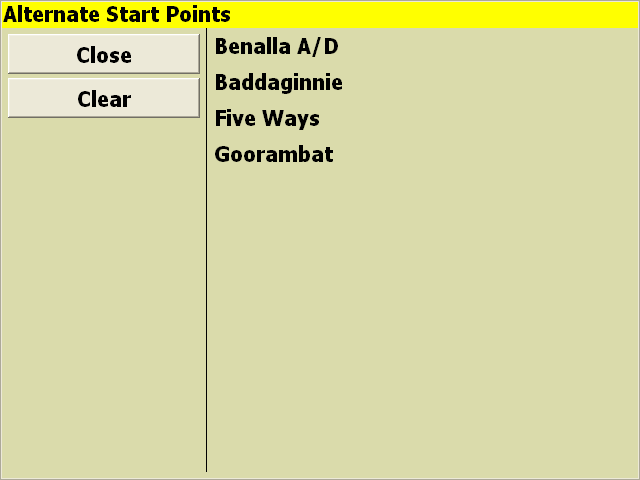
\includegraphics[angle=0,width=0.8\linewidth,keepaspectratio='true']{figures/dialog-startpoint2.png}
%\end{center}

%  To edit the start points, move the cursor to an item in the list on
%  the right side of the dialog, and press enter.  This opens the
%  waypoint selector dialog, to allow selection of the waypoint.  This
%  process can be repeated several times for several alternate start
%  waypoints.  Press the `clear' button to clear all alternate start
%  points.

%  Each start sector is fixed to the same type (line/cylinder) and size
%  (start radius) defined in the task waypoint page.

%  Note that the task start point should be included in the alternate
%  start location list.

%\begin{center}
%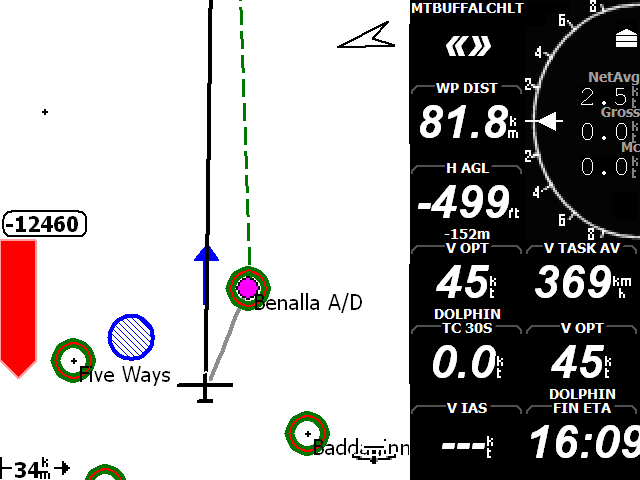
\includegraphics[angle=0,width=0.8\linewidth,keepaspectratio='true']{figures/dialog-startpoint3.png}
%\end{center}

%\begin{center}
%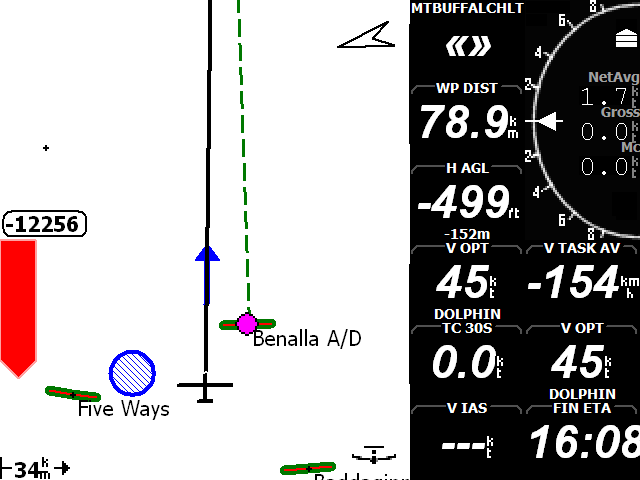
\includegraphics[angle=0,width=0.8\linewidth,keepaspectratio='true']{figures/dialog-startpoint4.png}
%\end{center}

%  In flight, any time you cross a start line (or exit a start
%  cylinder), this will start the task at that particular alternate
%  start.  Task statistics are recalculated for the start sector you
%  last flew through.  All alternate start sectors are shown on the
%  map.  You can re-start simply by flying through the start sector
%  again or another start sector.  This automatic re-start will only
%  happen if the active waypoint is the first turnpoint after the
%  start, or the start itself.

%  When the waypoint advance mode is `Arm' or `Arm Start', then a start
%  is only recognised by\textsf{XCSoar}  if the advance trigger is armed.

%  If desired, alternate start points may be selected as the active
%  waypoint by selecting the previous waypoint.  Continuing to select
%  the previous waypoint will cycle through all alternate start points.

\section{Aufgaben(Endanflug) Rechner-Fenster} \label{sec:task-calc-dial}\index{Aufgabe!Endanflugrechner)}
Im Rechner-Fenster der Aufgabenverwaltung werden einige Werte angezeigt, welche sich vor allem auf den Endanflug beziehen.

Dies Fenster kann aufgerufen werden wie folgt:
\begin{itemize}
\item Vom Hauptmenü mittels
\begin{quote}
\smenus{Nav}\blink\smenus{Aufgabe}\blink \button{Rechner}
\end{quote}
\item Aus der Analyse-Seite über \smenus{Info}\blink\smenus{Analysis}\blink\button{Aufgabenberechnung}
\end{itemize}

\begin{center}
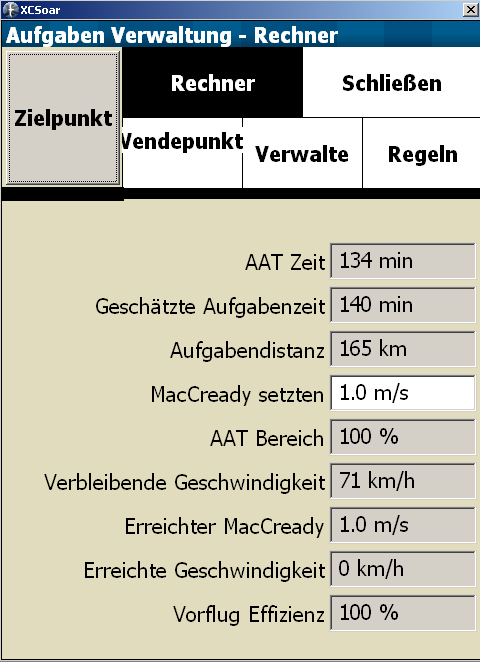
\includegraphics[angle=0,width=0.65\linewidth,keepaspectratio='true']{figures/dialog-taskcalc3.png}
\end{center}

\begin{description}
\item[AAT-Zeit]  Zeigt die der Aufgabe zugeordnete Mindest-Zeit an.
\item[Geschätzte Aufgabenzeit]  Zeigt die von \textsf{XCSoar} unter Berücksichtung der MC-Einstellung brechnete Zeit an, die Aufgabe zu beenden .
\item[Aufgabendistanz]  Zeigt die noch zu fliegende Distanz an.
\item[MacCready setzen]  Hier kann der MC-Wert verändert werden, um zu beobachten, wie sich damit die Aufgabenzeit ändert. \todonum{Zeigt nur die Gesamtzeit an. Schöner wäre auch die "Zeit drüber", dafür gibt es aber ja sinvollerweise die InfoBoxen\dots  !}
\item[AAT-Bereich] Erlaubt, den Bereich der Aufgaben zu variieren. \todonum{(? tut es nicht. Es zeigt nur an)}
\item[Verbleibende Geschwindigkeit]  Zeigt die zu fliegende Geschwindigkeit an, um den Task in der angegebenen Zeit gemäß der aktuellen MC-Einstellung zu fliegen.
\item[Erreichter MacCready]  Zeigt den in der Aufgabe erreichten gesamt erflogenen MC-Wert an.
\item[Vorflug Effizienz]  100\% steht für perfekten Vorflug bzw.\ Flug nach der MC-Theorie,  größer zeigt bessere Werte an (z.B.\ Fliegen unter Aufwindstraßen). Kleinere Werte zeigen, daß evtl. viel um den Kurs herumgeflogen wurde.
    Dieser Wert wird aus der seit dem Start erflogenen Performance berechnet und ständig aktualisiert.
\end{description}
Siehe auch~\ref{sec:task-speed-estim}.

Mit dem Schließen des Dialoges wird dieser MC-Wert für die weitere Berechnung benutzt.

Mit dem \button{Zielpunkt} Knopf, der ausschließlich für AAT Aufgaben gedacht ist, kann der entsprechende Wendepunkt innerhalb der AAT-Fläche verschoben werden.

 Die Wendepunkte können separat angewählt werden. Ist  "Auto" angeklickt, so berechnet \textsf{XCSoar} anhand der im  Hauptmenü eingestellten Delta-Zeit die optimal gelegenen Wendepunkte, wenn nicht, kann man den Wendepunkt manuell verschieben, solange bi die Ankunftszeit entsprechend des MC Wertes passend erscheint.
%
\section{Task Status Seite}
Der Task-\textbf{Status}-Dialog (s. Abschnitt~\ref{sec:dialog-windows}) bietet eine Übersicht über zum Teil  wichtige Informationen und den aktuellen Stand der Aufgabe (wie weit ist noch zu fliegen, welche Zeit ist noch "übrig", welcher mittlere Schnitt konnte erflogen werden  etc.\ ). Die Seite ist auch nützlich, um evtl. überflüssige oder nicht mehr benötigte InfoBoxen mit neuen Werten neu zu belegen. Weiterhin kann hier nochmals kontrolliert werden, ob z.B. ein gültiger Start der Aufgabe erkannt wurde.

Diese Seite kann über das folgende Menü aufgerufen werden:
\begin{center}
%\begin{quote}
\bmenu{Info}\blink\bmenu{Info}\blink\bmenu{Status}
%\end{quote}
\end{center}

\section{Assigned Area Aufgaben/Targets}\label{sec:aat-tasks}
\subsection*{AAT-Wendepunkte (targets)}\index{targets}
\index{AAT-Wendepunkte (targets)}

AAT-Wendepunkte werden in \textsf{XCSoar} gesondert behandelt und heißen  \textcolor[rgb]{0.00,0.00,0.50}{{\em Zielpunkt}}. Ein  {\em Zielpunkt } ist ein Wendepunkt innerhalb einer AAT Aufgabe, den der Pilot ausgewählt hat und anfliegen will. Es ist \textsl{nicht} der Wegpunkt, um den die AAT-Area gelegt ist, sondern der "echte" Wendepunkt.

Diese targets können innerhalb der AAT Aufgaben verschoben werden, wobei dem Piloten die Auswirkungen dieser Verschiebung in bezug auf Strecke, Delta Zeit (besonders wichtig), Ankunftszeit, Schnittgeschwindigkeit etc.\ unmittelbar klar dargestellt werden.  Targets können sowohl am Boden als auch in der Luft erstellt und verschoben werden.

Wenn eine AAT Aufgabe geflogen wird, rechnet das komplette Navigationssystem nicht auf den Mittelpunkt der AAT-Area, welcher z.B.\ von der Wettbewerbsleitung als Navigationspunkt gegeben ist, sondern explizit auf den vom Piloten festgelegten, evtl. verschobenen und  somit aktivierten Zielpunkt, das Zielpunkt.

Die automatische Wegpunkt-Weiterschaltung  funktioniert bei AAT-Aufgaben nicht, wenn der Pilot in die AAT-Area einfliegt. Der Pilot muß manuell  die Umschaltung zum nächsten Wegpunkt vornehmen, denn nur er weiß, wann wirklich gewendet worden ist. (Unmittelbar einleuchtend, denn \textsf{XCSoar} kann das nicht wissen\dots)

Wenn der vom Piloten gesetzte AAT-Zielpunkt umrundet und zum nächsten Zielpunkt gewechselt wurde, optimiert \textsf{XCSoar} nun für den Rest der Aufgabe. Siehe hierzu Abschnitt ~\ref{sec:advanc-rest-tasks} for details.

\subsection*{Manuelles verschieben der Ziele/Zielpunkte}

Um die größtmögliche Fläche bzw. Streckenausbeute der Aufgaben darzustellen, wird die Darstellung beim Verschieben der Zielpunkte  in \% angegeben.  So steht z.B. 100\% für das Maximum der Strecke, welche zum jeweiligen Zeitpunkt möglich ist, -100\% steht für die minimal mögliche Strecke, die zum jeweiligen Zeitpunkt erreicht werden kann. Die Berechnungen der \%-Werte erfolgen immer vom jeweiligen Standort aus.

Der Wert 0 wird erreicht, wenn exakt die vorgegebenen Punkte als Zielpunkt benutzt werden.  Handelt es sich bei den AAT-Areas um Sektoren, wird hierbei der Punkt am Ende der Winkelhalbierenden von An- und Abflugkurs  angenommen, sind Zylinder abzufliegen, wird der Mittelpunkt des Zylinders benutzt.

Der Aufgabenrechner, siehe~\ref{sec:task-calc-dial}, zeigt die mittlere Strecke der Aufgabe analog den oben gemachten Aussagen in \% und z.B. in Kilometer an.

Die Zielpunkte können individuell über den Zielpunkt-dialog geändert werden. Hierzu:

\begin{quote}
\bmenu{Nav}\blink\bmenu{NAV}\blink\bmenu{Zielpunkt}
\end{quote}

\subsection*{AAT targets und der Aufgabenrechner}

Hier soll ein typisches Verfahren zur Verwendung bzw. Arbeit mit targets innerhalb einer AAT-Aufgabe besprochen werden:
\begin{itemize}
\item Setze den erwarteten MacCready-Wert, Mücken und Wasserballast und stelle den Wind entsprechend ein.
\item Erstelle die Aufgabe ganz normal im Task Editor und markiere diese als Typ AAT.
\item  Die entsprechenden Wegpunkte müssen entsprechend markiert werden (TYP: Zylinder, Sektor , Zylinder mit innerem Radius o.ä)
\item Basierend auf den Einschätzungen des Piloten und der Güte des Wetters und auf der individuellen Erfahrung, ob manche Bereiche eher schwierig eingeschätzt werden (z.B. große Feuchtgebiete) können die targets manuell in jeder AAT-Area verschoben werden.
Im \textsf{ETE}-Feld des Aufgabenrechners kann einfach erkannt werden, ob die eingestellte Aufgabenzeit mit der entsprechenden Strecke korreliert und wie sich Änderungen durch Verschiebungen der targets auf die Ankunftszeit und die Deltazeit  auswirken.
\item Während des Fluges, wenn sich z.B.\ die Wettersituation ändert, und infolge der MC-Wert geändert werden muß,
    kann der Aufgabenrechner benutzt werden, um sich die nun  einstellende Situation anzeigen zu lassen, um vor allen eine zu frühe Ankunft zu vermeiden.
\item Alle Einstellungen bzgl. Ausdehnung oder Abkürzung der Aufgabe können über die Aufgabenverwaltung vorgenommen werden.
\item \textcolor[rgb]{0.00,0.25,0.50}{\textsf{Viel einfacher jedoch ist -vor allem im Fluge- der bereits oben erwähnte Aufruf von}}
\begin{center}
%\begin{quote}
\bmenu{Nav}\blink\bmenu{NAV}\blink\bmenu{Zielpunkt}
%\end{quote}
mit dem mit weniger Tip-Arbeit die AAT-targets problemlos verschoben und die Resultate bezgl.\ der Aufgabe insbesondere der Delta Zeit werden können.
\end{center}
\end{itemize}
Der Aufgabenrechner unterstützt den Piloten bei Fragestellungen wie z.B:\
\begin{itemize}
\item Was wird geschehen, wenn die Bedingungen besser werden?

Der MacCready kann dann angehoben, anschließend die targets nach außen verschoben werden (automatisch oder manuell, auch separat) um zu sehen, ob die Änderungen so passend sind, um die Aufgabe nun erfolgreich innerhalb der vorgegebenen Zeit zu vollenden.
\item Was geschieht, wenn die Bedingungen sich verschlechtern? Genau wie im obigen Falle, kann hier mittels Anpassen des MC-Wertes und Verschieben der targets in entsprechende Wetterfenster (\textsl{flieg dalang - woŽs gut aussieht\dots}) verschiedene Bedingungen während des Fluges durchgespielt werden.
\item Was passiert, wenn ich an dieser Stelle die AAT-Area verlasse und wende?
Mittels  \bmenu{NAV}\blink\smenut{Nächster}{Wendepunkt}  wird der aktuelle Standort als Wendepunkt genommen und alle folgenden Berechnungen werden  unverzüglich aktualisiert. Es wird zum nächsten Wendepunkt navigiert. Zurück geht es mit \bmenu{NAV}\blink\smenut{vorheriger}{Wendepunkt}
\end{itemize}

\subsection*{Zielpunkt - Projektion}

\textsf{XCSoar} analysiert kontinuierlich den Flugweg durch die AAT-Areas, um  die optimalen Punkte zu finden, welche die größtmögliche Strecke innerhalb der vorgegebenen Zeit zu fliegen.

Programm-Intern verschiebt  \textsf{XCSoar} automatisch die Punkte solange, bis anhand der bisher erflogenen Schnitte und MC-Werte die optimal anzufliegenden Punkte gefunden wurden.

In machen Umständen mag es sinnvoll sein, \textsf{XCSoar} die Punkte automatisch wählen zu lassen (natürlich nicht, wenn man in eine Regenfront hieneinföge\dots)
\begin{itemize}
\item Wenn sich das Flugzeug  in der AAT-Area befindet, wird der Zielpunkt innerhalb dieser Area auf einen gestrichelten
Kreisbogen  gesetzt, welcher vom Zielpunkt der nächsten anzufliegenden Area durch das Flugzeug geht und genausoweit entfernt vom Rand der Area ist,
wie der aktuell gewählte Zielpunkt vom Rand der  nächsten Area. D.h. alle Punkte, welche auf der eingezeichneten
Kreislinie liegen, haben die gleiche Akunftszeit zur Folge.

Der Sinn ist, es dem Piloten zu vereinfachen, auszuwählen, die AAT-Area mit einem Offset zum bisherigen Kurs oder aber in einem
anderen Winkel als beim vorherigen Zielpunkt in die Area einzufliegen. Sehr sinnvoll zum Beispiel, wenn man wolkenstraßenbedingt (gut oder schlecht \dots )
einen kleinen Haken schlagen muß, dennoch aber die Aufgabenzeit im Auge behalten muß.


\item Wenn sich das Flugzeug in der AAT-Area befindet und die Entfernung vom vorherigen Zielpunkt zum Flugzeug größer ist als die Entfernung vom vorherigen Zielpunkt zum nächsten Zielpunkt, wir der aktuelle Zielpunkt weiter entlang der Linie  bis zur Flugzeugposition verschoben.  Daher wird in diesem Falle die schwarze Kurslinie  nicht sichtbar sein, dafür aber wird der blaue Pfeil für den optimalen Kurs sichtbar werden. \footnote{Das ist sicher schön, aber ich verschiebe meine targets lieber selber - ins Wetter! IMHO no need for doing ist automatically}

\end{itemize}

Hier ein etwas detaillierteres Besipiel, um zu sehen, wie targets während  eines Fluges von \textsf{XCSoar} verschoben werden, um auf die Punkt optimiert Strecke zu fliegen

\todonum{Hier müssen unbedingt mal neue Bilder rein. Das stimmt alles so nicht mehr}
\begin{maxipage}
\begin{center}
\begin{longtable}{|c|c|}
\toprule
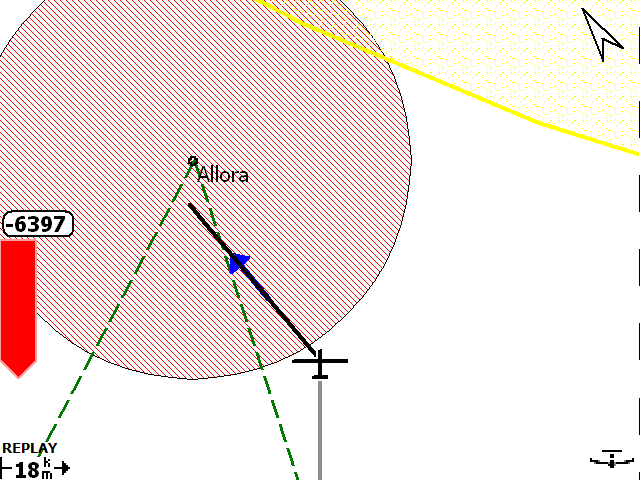
\includegraphics[angle=0,width=0.45\linewidth,keepaspectratio='true']{figures/faat01.png} &
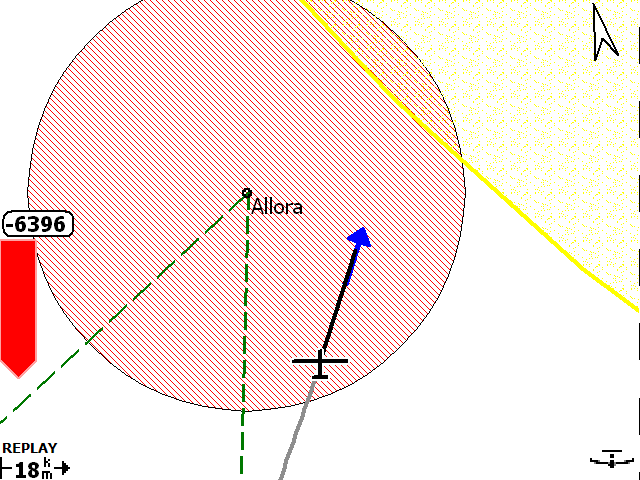
\includegraphics[angle=0,width=0.45\linewidth,keepaspectratio='true']{figures/faat02.png} \\
{\em Außerhalb des Sektors } & {\em Innerhalb des Sektors} \\
Zielpunkt (-20\%) ist auf der Winkelhalbierenden & Zielpunkt auf der Kurslinie \\

\midrule
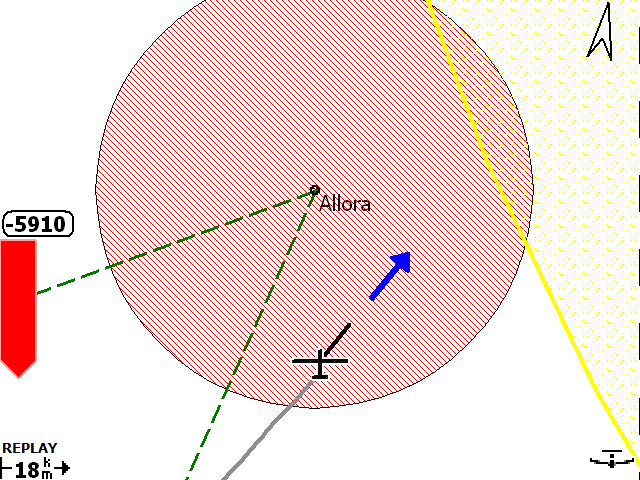
\includegraphics[angle=0,width=0.45\linewidth,keepaspectratio='true']{figures/faat03.png} &
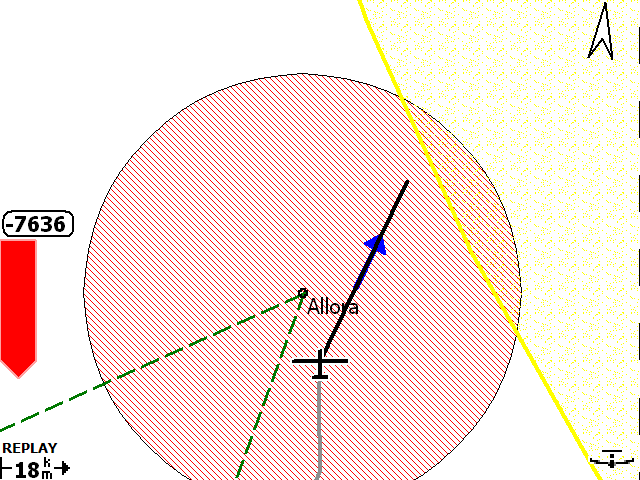
\includegraphics[angle=0,width=0.45\linewidth,keepaspectratio='true']{figures/faat04.png} \\
{\em Pilot hat die Reichweite verringert} & {\em Pilot hat Reichweite  vergößert} \\
Zielpunkt (-80\%) bewegt sich entlang der Kurslinie  & Zielpunkt (80\%) bewegt sich entlang Kurslinie \\

\midrule
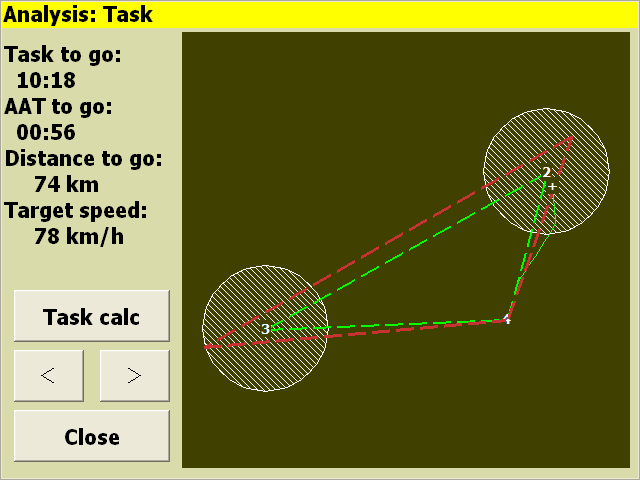
\includegraphics[angle=0,width=0.45\linewidth,keepaspectratio='true']{figures/faat05.png} &
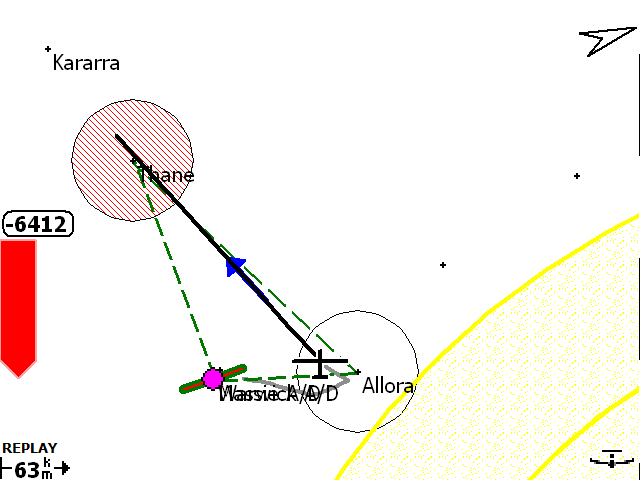
\includegraphics[angle=0,width=0.45\linewidth,keepaspectratio='true']{figures/faat06.png} \\
{\em Analyse (Aufgaben -Seite)} & {\em Nächster Wegpunkt} \\
Kurs rund um aktiven Zielpunkt & 'Nächster Wegpunkt' gedrückt\\
\bottomrule
\end{longtable}
\end{center}
\end{maxipage}

\begin{maxipage}
\begin{center}
\begin{longtable}{|c|c|}
\toprule
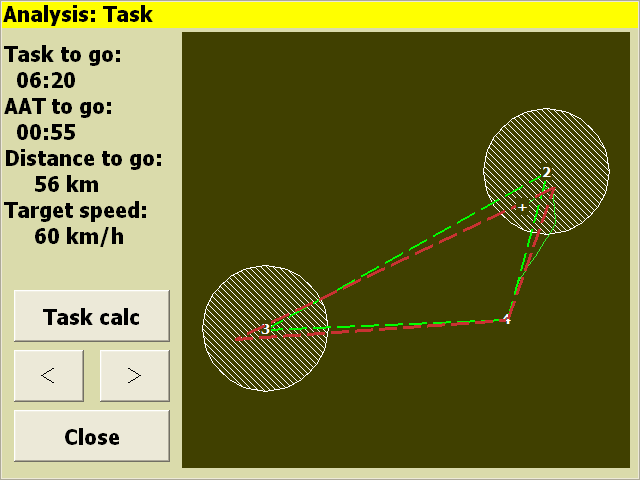
\includegraphics[angle=0,width=0.45\linewidth,keepaspectratio='true']{figures/faat07.png} &
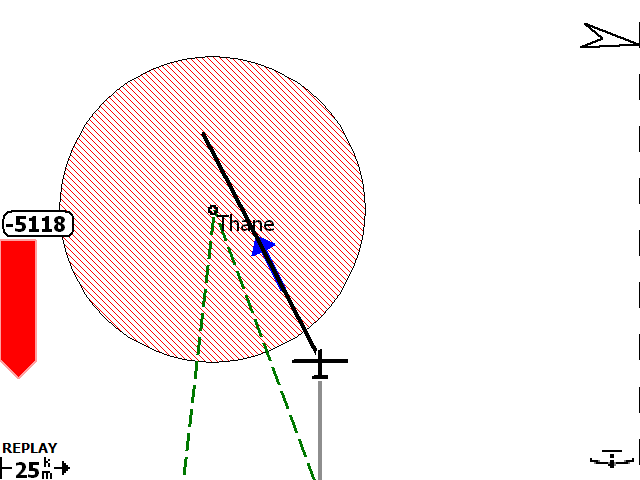
\includegraphics[angle=0,width=0.45\linewidth,keepaspectratio='true']{figures/faat08.png} \\
{\em Analysis (task page)} & {\em Approaching next area} \\
Optimaler Zielpunkt gefunden & Zielpunkt (60\%) ist auf Winkelhalbierender\\

\midrule
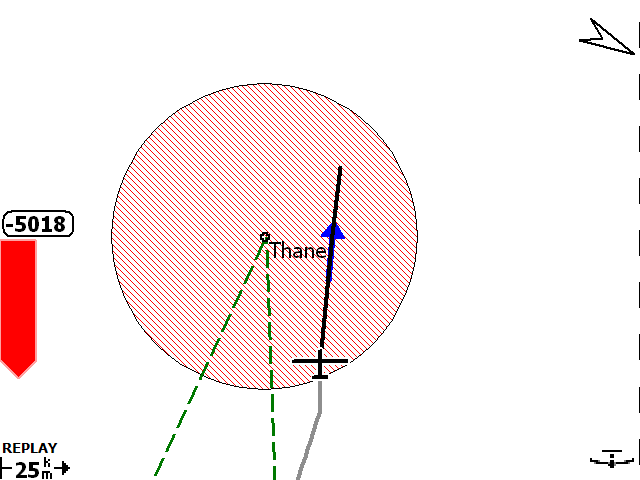
\includegraphics[angle=0,width=0.45\linewidth,keepaspectratio='true']{figures/faat09.png} &
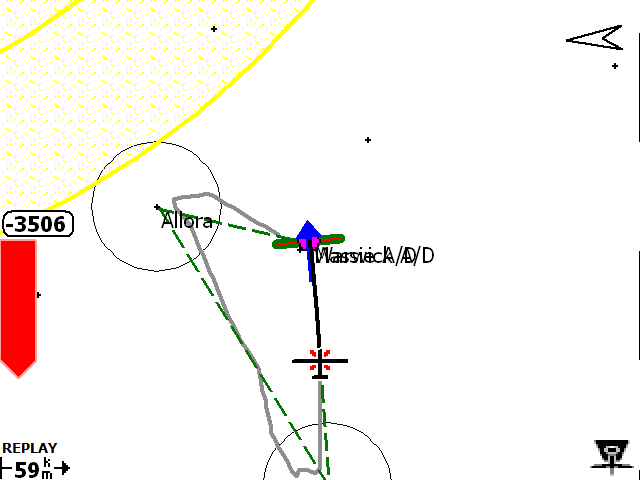
\includegraphics[angle=0,width=0.45\linewidth,keepaspectratio='true']{figures/faat11.png} \\
{\em Inside sector} & {\em Next waypoint} \\
Zielpunkt (60\%) entlang Kurs verschoben & ``Arm Turn" gedrückt\\

\midrule
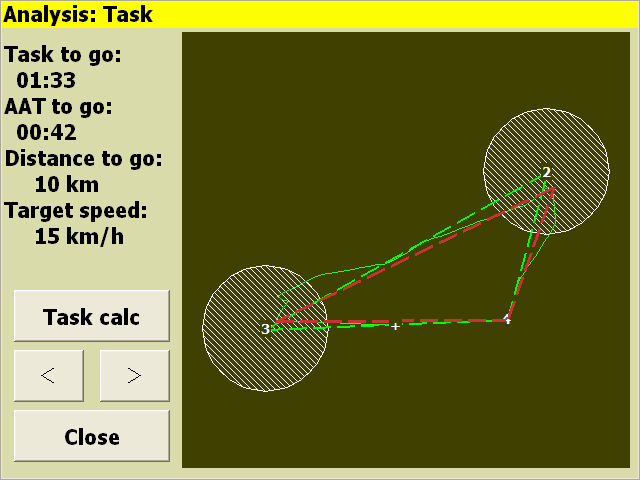
\includegraphics[angle=0,width=0.45\linewidth,keepaspectratio='true']{figures/faat12.png} &  \\
{\em Analysis (Aufgaben-Seite)} &  \\
Optimale Zielpunkte gefunden  &  \\

\bottomrule
\end{longtable}
\end{center}
\end{maxipage}

\section{OnLine-Contest OLC}

In diesem Dialog können OLC - optimierte settings abgespeichert werden, alle Infos zu OLC werden hier gezeigt. Die nach OLC gewertete Strecke und Punkte können abgerufen werden. Einstellungen können gemacht werden über  \config{taskrules} \index{OLC}

Während \textsf{XCSoar} läuft, wird kontinuierlich im Hintergrund nach den OLC Regeln optimiert, die Ergebnisse können  jederzeit  aufgerufen werden.
Auf der Analysis Seite wird eine graphische Übersicht der optimierten Ergebnisse Schnitt, Strecke und Punkte dargestellt.  Es besteht die Möglichkeit, die OLC-Werte (Strecke oder Punkte) auch in einer \infobox während es Fluges mitlaufen zu lassen

\begin{center}
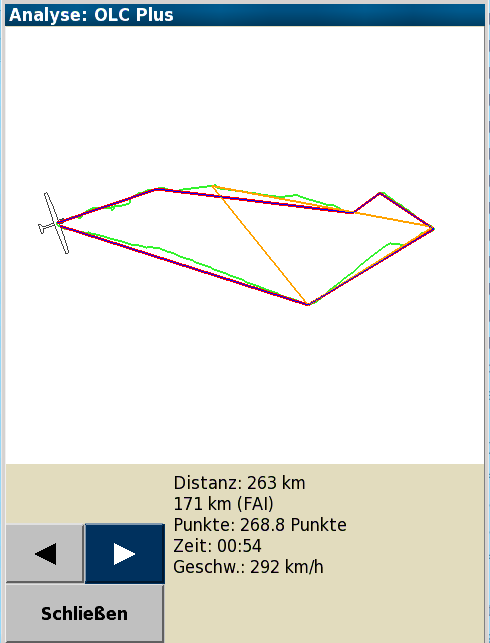
\includegraphics[angle=0,width=0.8\linewidth,keepaspectratio='true']{figures/shot-olc.png}
\end{center}

Es ist egal, ob AAT oder Nicht AAT Aufgaben geflogen werden, die interne OLC-Optimierung findet hiervon unabhängig gemäß der vorher gewählten Regeln statt.  Auf In der OLC Analyse-Seite wird der Flugweg als grün gestrichelter Linie dargestellt, der optimale Weg ist rot gestrichelt.

Wenn Flüge im Endanflug über das Ziel hinaus erweitert werden, werden die Ergebnisse als 'in Berechnung' angezeigt und eine blaue Linie zeigt den optimalen Kurs an, um das Maximum an Punkten zu erlangen.

Für OLC Sprint- und Classic-Aufgaben wird der Kurs einfach über das Ziel hinaus verlängert.  Für OLC-Dreiecksflüge wird dieser Kurs in eine Richtung vorgeschlagen, der das größtmögliche Dreieck ergibt.. \todonum{still true?}

Die Punktzahl und die kalkulierte, optimale Entfernung sind Näherungswerte.Nachdem das Flugzeug gelandet ist, werden keinerlei Werte mehr baufgezeichnet

\section{Aufgabenabbruch - Alternativen-Modus}\index{Außenlandung}\index{Aufgabenabbruch}

Wenn sich die Thermikbedingungen derart verschlechtern, daß die Aufgabe nicht mehr fortgesetzt werden kann,
dann es ist mittels des Aufgabenabbruchs möglich, \textsf{XCSoar} auf eine Art 'Notfall-Navigation' umzustellen.
Hierbei werden alle navigatorischen Berechnungen der aktuellen Aufgabe abgebrochen und die Priorität auf sicheres
Erreichen eines nahe gelegenen Flugfeldes gelegt.

Um in diesen Modus zu gelangen, drücke:
\begin{quote}
\bmenu{Nav}\blink\bmenu{Nav}\blink\bmenut{Aufgabe}{abbruch}
\end{quote}

Wenn dies gewählt wurde,  ist jede Aufgabe, was immer auch vorher programmiert, abgebrochen.
Die Berechnung der Landefelder erfolgt unter Berücksichtigung des eingestellten Sicherheits MC-Wert.

Die Aufgaben-Wegpunkliste ist nun gefüllt mit den nächsten zu erreichenden Flugplätzen, sortiert gemäß den Angaben
der  "Alternativen-Modus" in den Konfigurations -Einstellungen \config{alternatesmode}

Die Anzeige wechselt in der Art, als daß ausschließlich mit der derzeit vorhandenen Höhe erreichbare
Landefelder angezeigt werden. Das Verhalten, welche Landefelder in welcher Priorität angezeigt werden, kann unter

\begin{quote}
\bmenu{Konf.}\blink\bmenu{Konf.}\blink\bmenut{System}{Einstellungen}
\end{quote}

Auf der Seite

\begin{quote}
\bmenu{Sicherheitsfaktoren}\blink\bmenu{Endanflug}\blink\bmenu{Alternativen Modus}
\end{quote}

voreingestellt werden. Folgende Optionen sind dabei möglich:
\begin{description}
\item[Einfach] Alternativen werden lediglich nach Wegpunkt-Typ und Ankunftshöhe sortiert.
Die angenommene Ankunftshöhe wird unter Berücksichtigung des Windes mittels des Sicherheits  MC-Einstellung vorgenommen.
Der erste Punkt in der Liste  ist der am sichersten Erreichbare.
\item[Aufgabe] Zusätzlich zu den oben genannten Bedingungen wird hier die Kursrichtung zum programmierten \textbf{Zielpunkt} berücksichtigt, um im Falle einer
Wiederaufnahme der Aufgabe optimal weiterfliegen zu können, ohne Haken schlagen zu müssen.
\item[Heimat] Der Sortieralgorythmus wird bevorzugt jene Felder auswählen, die auf dem Kurs in Richtung des \textbf{Heimatflugplatzes} liegt.
\end{description}

Die Konfigurations-Option "Abort use current MC"\todonum{find ich in V64 nicht mehr}  entscheidet darüber,
ob die Ankunftshöhe gemäß des manuell eingestellten MC-Wertes oder aber der mit Hilfe des
Sicherheits MC-Wertes durchgeführt wird.

Als Standard ist der Sicherheits-MC Wert eingestellt. \index{Sicherheits-MC-Wert}\index{MC-Cready!Sicherheits}
Wenn in den Abbruch-Modus gewechselt wird, wird der Sicherheits MC-Wert genommen, sofern er kleiner ist als der aktuell
manuell eingestellte oder ermittelte Wert.

Wenn kein Landefeld/Flugplatz erreichbar ist, werden die nächsten 10 als landbar markierten Plätze angezeigt.

\begin{center}
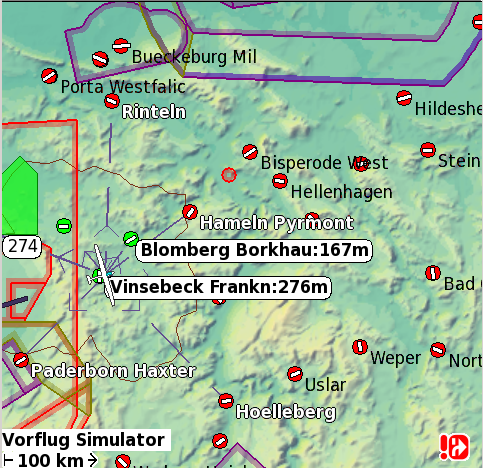
\includegraphics[angle=0,width=0.8\linewidth,keepaspectratio='true']{figures/abort-low.png}
\end{center}

Wenn mindestens ein landbarer Punkt erreichbar ist, dann wird einzig dieser Punkt angezeigt.\todonum{Kontrolle stimmt das?}

\begin{center}
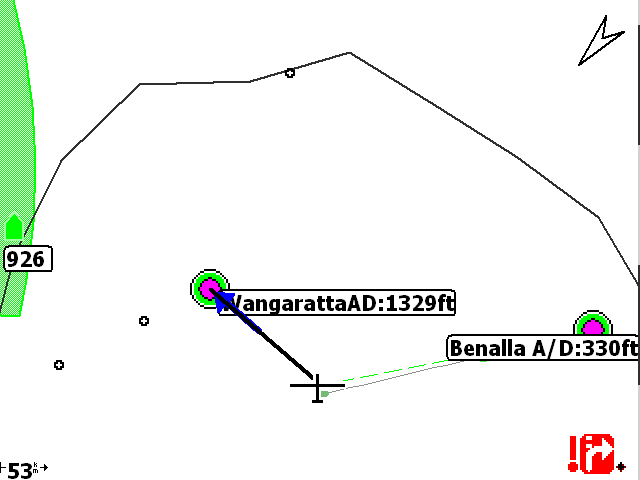
\includegraphics[angle=0,width=0.8\linewidth,keepaspectratio='true']{figures/abort-high.png}
\end{center}

Wenn der Wegpunkt, welcher vor dem Aufgabenabbruch aktiv war, landbar ist und erreichbar erscheint,
dann bleibt dieser Wegpunkt auch im Aufgabenabbruch-Modus der aktive.
Andernfalls wird der allernächste landbare  Wegpunkt als aktiver Wegpunkt benutzt - auch wenn es
keine erreichbaren Wegpunkte gibt.
\todonum{HÄ ??  nochmal drüberlesen }

Der aktive  Wegpunkt und auch die Liste der nahen landbaren Punkte innerhalb der Aufgabe werden im Aufgabenabbruch-Modus dynamisch aktualisiert, so daß der Pilot ständig eine aktuelle Übersicht von Landeoptionen hat.  Jede dieser Optionen kann  mit dem 'FliegHin' zum aktiven Wegpunkt deklariert und benutzt werden.

Es ist jederzeit mittels

\begin{quote}
\bmenu{Nav}\blink\bmenu{Nav}\blink\bmenut{Aufgabe}{Fortsetzen}
\end{quote}

die Aufgabe wieder herzustellen, sollte sich das Wetter wieder erholen.
Alle Daten wurden intern zwischengespeichert und die Navigation geht nun weiter, als "wäre nichts gewesen".
%
\textcolor[rgb]{0.00,0.25,0.50}{\textsf{Wenn im Aufgabenabbruch-Modus geflogen wird, geht der Rechner automatisch in den  Endanflug-Modus.}}
%
\section{Logger}

Ein IGC konformer Logger kann problemlos mit \textsf{XCSoar} verbunden werden, um Flüge gemäß IGC aufzuzeichnen. die folgenden werden derzeit unterstützt:

\begin{itemize}
\item Ein software basierter Logger.  Alle Versionen von\textsf{XCSoar}  besitzen diese Funktionalität.  Dieser Logger ist IGC - konform, aber derzeit noch nicht IGC-zugelassen.
\item Die Pro Version des Altair hat einen internen IGC logger integriert.
\textsf{XCSoar} kommuniziert mit den Loggern genauso, als ob es sich um externe, serielle Geräte handelt.
\item\textsf{XCSoar} kann auch Deklarationen in Richtung externer Logger senden, um Aufgaben IGC-konform zu deklarieren. (Auch an Flarm!)

Damit dies funktioniert, muß das Gerät unter "Geräte" spezifiziert werden. \config{comdevices} settings.
\end{itemize}

Der interne Logger kann manuell oder automatisch eingeschaltet werden:

\todonum{stimmt das überhaupt noch ?}
\begin{quote}
\bmenu{Konfig.}\blink\bmenu{Konfig.}\blink\bmenu{Logger Start}
\end{quote}

Wenn der interne Logger aktiv ist und aufzeichnet, ist ein kleiner Diamant
in der rechten unteren Ecke des Displays zu sehen, der einmal pro Sekunde auf leuchtet

Standardmäßig schaltet\textsf{XCSoar}  automatisch den internen Logger ein und aus, sobald ein Flugzeugstart bzw.\ eine Landung  detektiert wurde.
Nur, wenn der Logger manuell gestartet wurde, fragt \textsf{XCSoar} nach, ob der Flug auch deklariert wurde. Beim automatischen Start wird der Flug automatsich deklariert.

Falls eine Aufgabe deklariert wurde, wird bei jeder Änderung, welche an der Aufgabe vorgenommen wird, nachgefragt, ob die Änderung ebenfalls in die Deklaration übernommen werden soll. Dies, um bei der Deklaration die Übersicht zu behalten, falls etwas geändert wurde, ohne es abzuspeichern.

Der\textsf{XCSoar}  Software - Logger überprüft bei jedem Start, ob mindestens 500kB Speicherplatz frei ist, um eine fehlerfreie Aufzeichnung zu gewährleisten. \textcolor[rgb]{0.00,0.25,0.50}{Ist nicht genügend Speicherplatz auf dem Medium vorhanden, so wird automatisch der älteste auf dem Medium vorhandene IGC File gelöscht, ohne den Piloten hiernach zu fragen.}

Intern werden die aufgezeichneten Daten für 60sec. gepuffert, bevor die Aufzeichnung auch wirklich gestartet wird.  Dadurch wird gewährleistet, daß der Logger auf jeden Fall auch den kompletten Startvorgang mit aufzeichnet

\section{Logger Wiedergabe}
Flüge die im IGC Format von\textsf{XCSoar} aufgenommen wurden,  können   auch wieder abgespielt werden. Das Abspielen von gespeicherten Flügen erfolgt über:

\begin{quote}
\bmenu{Konfig.}\blink\bmenu{Konfig.}\blink\bmenu{Wiedergabe}
\end{quote}

\begin{center}
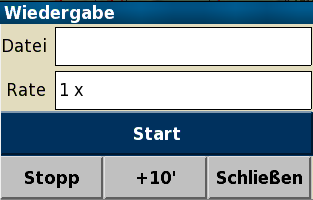
\includegraphics[angle=0,width=0.7\linewidth,keepaspectratio='true']{figures/loggerreplay.png}
\end{center}

Während der Wiedergabe erscheint ein "RREPLAY'' an der linken unteren Ecke des Displays.
\index{Wiedergabe aufgezeichneter Flüge}\index{Replay}
Um einen aufgezeichneten Flug zu starten, zuerst das File laden und anschließend auf \button{Start} drücken. Anschließend \button{Schließen}. Die Wiedergabe kann auch beschleunigt dargestellt werden, hierzu den entsprechend Faktor  (0x, 1x, 2x \dots 10x).
 ine Eingabe von 0 bewirkt das Pausieren der Wiedergabe.

Größere Werte für die Wiedergabegeschwindigkeit können(werden) eine reduzierte Detailtreue  bestimmter Flugdetails bewirken, wie z.B. die Aktualisierung des Windes und anderer in Echtzeit berechneter Routinen (Ablage, Thermikstärke).

Stoppen der Wiedergabe mit  \button{Stop}.
Wenn eine Aufzeichnung gestartet wurde, bewirkt ein erneutes Drücken auf \button{Start} einen Neustart der Wiedergabe.

Anmerkung:

Es wird empfohlen, einen \textsl{RESET}  des  Gerät vor einem erneuten Flug durchzuführen, um sicherzustellen, daß die internen Statistiken von \textsf{XCSoar} regelgerecht zurückgesetzt wurden -dies ist unter anderem Betriebssystembedingt.

Wenn \textsf{XCSoar} im Flug-modus betrieben wird, ist der Replay Modus deaktiviert und kann auch nicht aktiviert werden, sobald ein echter GPS Empfänger detektiert wird.

Die Wiedergabe der aufgezeichneten Flüge funktioniert am besten mit relativ hohen Aufzeichnungsraten, 6 Sekunden oder weniger werden hier empfohlen.

\section{Analysis dialog}\label{sec:analysis-dialog-climb}

Die Analyse Seite ist recht hilfreich um den bisherigen oder komplett geflogenen Flug komplett zu "durchleuchten".  Aufgerufen wird der Dialog mit
\begin{quote}
\bmenu{Info}\blink\bmenu{Analyse}
\end{quote}

Auf diversen Seiten kann nach etlichen Details  des Fluges gesucht werden:
\begin{description}
\item[Barograph]  Zeigt das Barogramm des Fluges.

Die Statistiken hier können genutzt werden, um die Arbeitshöhe zu ermittlen und wie sich z.B.\  die Arbeitshöhe bzw. die Basis über die Zeit ändert. Die Basis und Bedeckung ist in das Barogramm eingezeichnet (die Basis kann unter   eingestellt werden)

\button{Einstellungen}  öffnet den Flug-Einstellungen - Dialog.
  (z.B. zum einstellen des QNH, Ballast, mücken oder der max.\ Temperatur)

\begin{center}
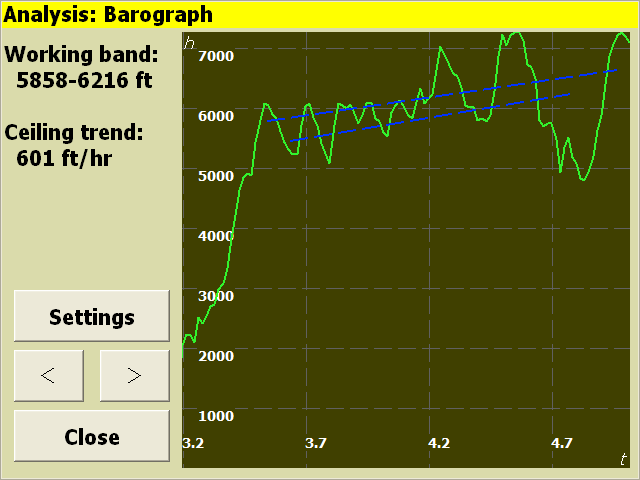
\includegraphics[angle=0,width=0.8\linewidth,keepaspectratio='true']{figures/analysis-barograph.png}
\end{center}

\item[Steigen]
  Zeigt den Verlauf der bisher erfolgenen Bärte.
  Diese Statistik kann benutzt werden, um z.B. den Schnitt aller Bärte des Tages herauszufinden, oder wie sich die Entwicklung über den Verlauf des Fluges änderte.

  Der aktuell eingestellte MC-Wert  ist zum Abgleich als dicke, rot-getrichelte Linie eingezeichnet, der Steigwert ist als blaue Linie im Diagramm enthalten.


\begin{center}
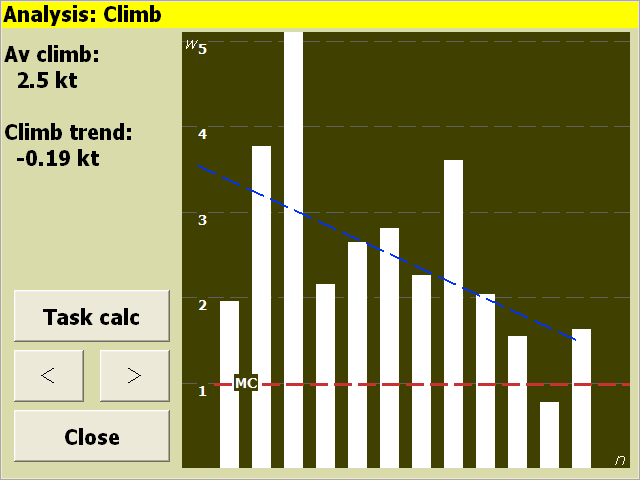
\includegraphics[angle=0,width=0.8\linewidth,keepaspectratio='true']{figures/analysis-climb.png}
\end{center}

\item[Aufgabe]
Diese Seite zeigt einen schematischen Überblick über die gesamte Aufgabe (ohne Karte im Hintergrund).
Blauviolett dargestellt ist die Kartenkurslinie, AAT-Areas sind gelb hinterlegt. Der geflogene Kurs ist grün dargestellt.

Mit \smenut{Aufgabe}{Berechnung} kommt man direkt in die Aufgabenverwaltung.

\item[Luftraum]
Eine Übersicht über die im Task über- unter, oder durchflogenen Lufträume wird als Grafik über der Zeitachse dargestellt.Lufträume sind als Markierungen mit seitlicher und ober Höhe  dargestellt.

Weitere Seiten, die hier aufgeschlagen werden können,  sind z.B. Konvektionshöhe mit einer Darstellung der erflogenen Basishöhe

\todonum{Wie hängen diese Diagramme  mit z.B. den rasp Vorherrsagen zusammen ? Werden die mit aktualisiert? oder wird lediglich das bartende als z.B. Basis bewertet ?}
\begin{center}
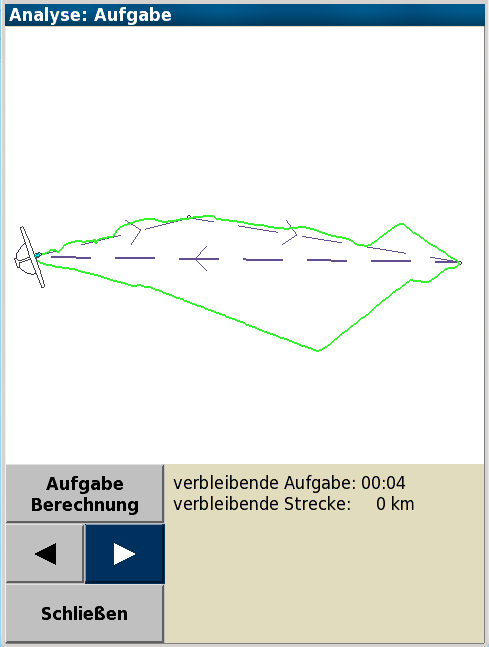
\includegraphics[angle=0,width=0.8\linewidth,keepaspectratio='true']{figures/analysis-task.png}
\end{center}
\end{description}

\section{Sonneneinstrahlung und -dauer}

Eine Sonnenscheindauer und -standroutine berechnet den Sonnenuntergang, welcher im Luftfahrzeugstatus-Dialog angezeigt wird. (siehe Abschnitt~\ref{sec:status}).

 Sowohl die geographische Lage, als auch  lokale Geländebeschaffenheiten und die atmosphärischen Bedingungen können zu einer Beeinträchtigung der Ablesbarkeit auch vor dem errechneten Sonnenuntergang führen kann.  \todonum{was soll dieser Satz? Überflüssig\dots}

Bei PDA-Systemen wird die Sommer- und Winterzeit automatisch nachgeführt, entsprechend der Einstellungen des Betriebssystems. Beim Altair, muss diese nach Führung im Konfigurationsmenü manuell durchgeführt werden.

Wenn die erwartete Ankunftszeit am Zielpunkt nach Sonnenuntergang liegt, erscheint eine Statusmeldung mit dem Hinweis darauf (z.B. "Erwarte Ankunft nach Sonnenuntergang").

\section{\textcolor[rgb]{1.00,0.00,0.00}{Heimatflugplatz}}
Wenn der Heimatflugplatz über den Wegpunkt-Info-Dialog (auf der zweiten Seite) eingegeben wird, benutzt \textsf{XCSoar} diesen Wegpunkt grundsätzlich beim Starten, sofern keine Aufgabe aktuell geladen ist, keine Standard Aufgabe erstellt und gespeichert wurde oder aber die Aufgabe abgebrochen wird. \index{Heimatflugplatz}
